% =============================================================================
%  lec26.tex —— 第 26 讲 ∞-操作子的张量积（底本 PDF 第 193–198 页）
% =============================================================================
\lecture{26}{$\infty$-操作子的张量积}
\begin{center}\small\color{black!55}（底本 PDF 第 193–198 页）\end{center}

本讲介绍 $\infty$-操作子的张量积。想法是：在 $\mathrm{Op}_{\infty}$ 上有一个对称幺半结构 $\odot$，使得对任意对称幺半 $\infty$-范畴 $\cC$，都有
\[
\Alg_{O_{1}}(\Alg_{O_{2}}(\cC))\simeq\Alg_{O_{1}\odot O_{2}}(\cC).
\]

\yizhu{本讲用 $\odot$ 专指 $\infty$-操作子之间的张量积，以区别于对称幺半 $\infty$-范畴内部的张量积 $\otimes$。这一记号沿用 Lurie 的 HA（即本讲定理—定义~\ref{L26-1.10} 所引的 HA.2.2.5.7）。\textbf{[来源：A]}}

\section{定义}

\nitem\label{L26-1.1} 回忆 $\mathrm{Op}_{\infty}$ 是 $(\Cat_{\infty})_{/\mathrm{Fin}_{*}}$ 的 \textbf{1-全}子 $\infty$-范畴。我们先在 $\mathrm{Fin}_{*}$ 上构造一个对称幺半结构。

\begin{construction}\label{L26-1.2}
回忆 $\Spc_{*}$ 具有由带基点空间的 smash 积给出的对称幺半结构 $(\Spc_{*})^{\wedge}\to\mathrm{Comm}^{\otimes}$。设 $(\mathrm{Fin}_{*})^{\wedge}\subseteq(\Spc_{*})^{\wedge}$ 为由满足「每个 $X_{k}$ 都是 $\mathrm{Fin}_{*}\subseteq\Spc_{*}$ 中的对象」的对象 $(X_{1},\cdots,X_{n})$ 构成的全子范畴。容易看出，$(\mathrm{Fin}_{*})^{\wedge}\to\mathrm{Comm}^{\otimes}$ 把 $\mathrm{Fin}_{*}$ 展示为一个对称幺半普通范畴，其乘法函子由
\[
-\wedge-\colon\mathrm{Fin}_{*}\times\mathrm{Fin}_{*}\to\mathrm{Fin}_{*},\qquad
(\langle m\rangle,\langle n\rangle)\mapsto\langle mn\rangle
\]
给出。换言之，我们得到对象
\[
\mathrm{Fin}_{*}\in\Alg_{\mathrm{Comm}}(\Cat_{\infty}),
\]
其中 $\Cat_{\infty}$ 配备笛卡尔对称幺半结构。
\end{construction}

\begin{exercise}\label{L26-1.3}
显式构造对称幺半范畴 $(\mathrm{Fin}_{*},\wedge)$，即给出结合子、单位子与换位自然变换。
\end{exercise}

\nitem\label{L26-1.4} 下一步是利用 $\mathrm{Fin}_{*}$ 上的对称幺半结构，在 $(\Cat_{\infty})_{/\mathrm{Fin}_{*}}$ 上构造对称幺半结构。这个构造对任意切片 $\infty$-范畴都适用。

\nitem\label{L26-1.5}\textbf{命题—构造}（HA.2.2.2.4）\quad 设 $\cC^{\otimes}\to\mathrm{Comm}^{\otimes}$ 是任意 $\infty$-操作子，$A\in\Alg_{\mathrm{Comm}}(\cC)$ 是交换代数。则存在典范的 $\infty$-操作子 $(\cC_{/A})^{\otimes}$，配备 $\infty$-操作子映射
\[
q\colon(\cC_{/A})^{\otimes}\to\cC^{\otimes},
\]
使得
\begin{enumerate}[label=(\arabic*),leftmargin=2.4em,itemsep=0.1em]
\item $\infty$-范畴 $(\cC_{/A})^{\otimes}_{\langle1\rangle}$ 等同于 $\cC_{/A(\langle1\rangle)}$。
\item $(\cC_{/A})^{\otimes}$ 中的态射 $f$ 是惰性的，当且仅当 $q(f)$ 是惰性的。
\item 若 $\cC^{\otimes}$ 是对称幺半的，则 $(\cC_{/A})^{\otimes}$ 也是，且 $q$ 是对称幺半函子。
\end{enumerate}

\begin{remark}\label{L26-1.6}
非形式地说，对对象 $M\in\cC_{/A}$ 与 $N\in\cC_{/A}$，它们的张量积是 $\cC_{/A}$ 中由复合
\[
M\otimes N\to A\otimes A\to A
\]
给出的对象。
\end{remark}

\begin{remark}\label{L26-1.7}
事实上，即使把 $\mathrm{Comm}^{\otimes}$ 换成一般 $\infty$-操作子 $\OO^{\otimes}$，类似的构造仍然存在。
\end{remark}

\nitem\label{L26-1.8} 特别地，对象 $\mathrm{Fin}_{*}\in\Alg_{\mathrm{Comm}}(\Cat_{\infty})$ 在 $(\Cat_{\infty})_{/\mathrm{Fin}_{*}}$ 上诱导一个对称幺半结构。

\begin{warning}\label{L26-1.9}
这不是 $(\Cat_{\infty})_{/\mathrm{Fin}_{*}}$ 上的笛卡尔对称幺半结构。
\end{warning}

\begin{theoremdef}\label{L26-1.10}（HA.2.2.5.7\footnote{在 HA.2.2.5.7 中，Lurie 实际构造的是 $\infty$-预操作子（$\infty$-preoperad）所成模型范畴上的对称幺半结构。展开定义可见，这个对称幺半模型范畴的底层对称幺半 $\infty$-范畴等价于 $(\mathrm{Op}_{\infty})^{\odot}$。}）
设
\[
(\mathrm{Op}_{\infty})^{\odot}\subseteq((\Cat_{\infty})_{/\mathrm{Fin}_{*}})^{\otimes}
\]
为满足下述条件的 \textbf{1-全}子 $\infty$-范畴：
\begin{enumerate}[label=(\roman*),leftmargin=2.4em,itemsep=0.1em]
\item 对象 $(C_{1},\cdots,C_{n})$ 含于 $(\mathrm{Op}_{\infty})^{\odot}$，当且仅当每个 $C_{k}\to\mathrm{Fin}_{*}$ 都是 $\infty$-操作子；
\item 定义在 $\alpha\colon\langle m\rangle\to\langle n\rangle$ 之上的态射 $(C_{1},\cdots,C_{m})\to(D_{1},\cdots,D_{n})$ 含于 $(\mathrm{Op}_{\infty})^{\odot}$，当且仅当对每个 $j\in\langle n\rangle^{\circ}$，相应的函子
\begin{equation}\label{L26-eq1.1}
\prod_{i\in\alpha^{-1}(j)}C_{i}\to D_{j}
\end{equation}
在每个因子上保持惰性态射。
\end{enumerate}
则 $(\mathrm{Op}_{\infty})^{\odot}\to\mathrm{Comm}^{\otimes}$ 使 $\mathrm{Op}_{\infty}$ 具有对称幺半结构。我们把该乘法函子记为
\[
(\mathrm{Op}_{\infty})^{\odot}\times(\mathrm{Op}_{\infty})^{\odot}\to(\mathrm{Op}_{\infty})^{\odot},\qquad
(\OO^{\otimes},\OO^{\prime\otimes})\mapsto(\OO\odot\OO^{\prime})^{\otimes}.
\]
\end{theoremdef}

\begin{remark}\label{L26-1.11}
条件 (ii) 等价于：函子~\eqref{L26-eq1.1} 把任意满足「每个 $f_{i}$ 都是 $C_{i}$ 中惰性态射」的态射 $(f_{i})_{i\in\alpha^{-1}(j)}$ 送到 $D_{j}$ 中的惰性态射。事实上，这由惰性态射对复合封闭推出。
\end{remark}

\nitem\label{L26-1.12} 与 Lurie 张量积的情形类似，对 $\infty$-操作子 $\OO_{i}^{\otimes}\in\mathrm{Op}_{\infty}$，存在典范函子
\[
\prod_{i=1}^{n}\OO_{i}^{\otimes}\to\Bigl(\bigodot_{i=1}^{n}\OO_{i}\Bigr)^{\otimes},
\]
它定义在 $\prod_{i=1}^{n}\mathrm{Fin}_{*}\xrightarrow{\wedge}\mathrm{Fin}_{*}$ 之上，并在每个因子上保持惰性态射。

\begin{exercise}\label{L26-1.13}
对任意 $C^{\otimes}\in\mathrm{Op}_{\infty}$，与上述函子复合，诱导出下述空间之间的等价：
\begin{itemize}[leftmargin=2.2em,itemsep=0.1em]
\item $\infty$-操作子映射 $(\bigodot_{i=1}^{n}\OO_{i})^{\otimes}\to C^{\otimes}$；
\item 定义在 $\prod_{i=1}^{n}\mathrm{Fin}_{*}\xrightarrow{\wedge}\mathrm{Fin}_{*}$ 之上、且在每个因子上保持惰性态射的函子 $\prod_{i=1}^{n}\OO_{i}^{\otimes}\to C^{\otimes}$。
\end{itemize}
若考虑这些函子构成的 $\infty$-范畴，同样的结论也成立。
\end{exercise}

\section{与 $\mathrm{Triv}^{\otimes}$、$E_{0}^{\otimes}$ 及 $\mathrm{Comm}^{\otimes}$ 作张量积}

\begin{exercise}\label{L26-2.1}
证明 $\mathrm{Triv}^{\otimes}\in\mathrm{Op}_{\infty}$ 是单位对象。
\end{exercise}

\begin{exercise}\label{L26-2.2}
证明
\[
(E_{0}\odot E_{0})^{\otimes}\simeq E_{0}^{\otimes},\qquad
(\mathrm{Comm}\odot\mathrm{Comm})^{\otimes}\simeq\mathrm{Comm}^{\otimes}.
\]
\end{exercise}

\begin{proposition}\label{L26-2.3}（HA.2.3.1.9）
显然函子 $\mathrm{Triv}^{\otimes}\to E_{0}^{\otimes}$ 使 $E_{0}^{\otimes}$ 成为 $\Alg^{\mathrm{idem}}_{\mathrm{Comm}}(\mathrm{Op}_{\infty})$ 中的对象，并且
\[
\Mod^{\mathrm{Comm}}_{E_{0}^{\otimes}}(\mathrm{Op}_{\infty})\subseteq\mathrm{Op}_{\infty}
\]
恰好由带单位 $\infty$-操作子构成。特别地，后者对 $\odot$ 封闭。
\end{proposition}

\yizhu{上标 $\mathrm{idem}$ 表示幂等：交换代数 $A$ 若其乘法 $A\otimes A\to A$ 是同构，则称为\textbf{幂等}的；$\Alg^{\mathrm{idem}}$ 表示由幂等代数构成的全子 $\infty$-范畴。这里 $\mathrm{Triv}^{\otimes}\to E_{0}^{\otimes}$ 使 $E_{0}^{\otimes}$ 成为 $\mathrm{Op}_{\infty}$ 中的幂等交换代数，因此可以谈论它上面的模。\textbf{[来源：B]}}

\begin{proposition}\label{L26-2.4}（HA.3.2.4.6）
显然函子 $\mathrm{Triv}^{\otimes}\to\mathrm{Comm}^{\otimes}$ 使 $\mathrm{Comm}^{\otimes}$ 成为 $\Alg^{\mathrm{idem}}_{\mathrm{Comm}}(\mathrm{Op}_{\infty})$ 中的对象，并且
\[
\Mod^{\mathrm{Comm}}_{\mathrm{Comm}^{\otimes}}(\mathrm{Op}_{\infty})\subseteq\mathrm{Op}_{\infty}
\]
恰好由余笛卡尔 $\infty$-操作子构成。特别地，后者对 $\odot$ 封闭。
\end{proposition}

\begin{exercise}\label{L26-2.5}
证明 $C^{\sqcup}$ 与 $D^{\sqcup}$ 的张量积等价于 $(C\times D)^{\sqcup}$。
\end{exercise}

\section{代数中的代数}

\nitem\label{L26-3.1} 现在我们转向等价
\[
\Alg_{O_{1}}(\Alg_{O_{2}}(\cC))\simeq\Alg_{O_{1}\odot O_{2}}(\cC).
\]
第一项任务是定义 $\infty$-操作子 $\Alg_{O_{2}}(\cC)^{\otimes}$。

\begin{construction}\label{L26-3.2}
设 $O_{1}^{\otimes},O_{2}^{\otimes}\in\mathrm{Op}_{\infty}$，且 $(O_{1}\odot O_{2})^{\otimes}\to O^{\otimes}$ 是 $\infty$-操作子映射。考虑对应
\[
O_{1}^{\otimes}\xleftarrow{p}O_{1}^{\otimes}\times O_{2}^{\otimes}\xrightarrow{m}O^{\otimes}.
\]
对任意 $O^{\otimes}$ 上的 $\infty$-操作子 $\cC^{\otimes}\to O^{\otimes}$，令
\[
\Alg_{O_{2}/O}(\cC)^{\otimes}\subseteq p_{*}\circ m^{*}(\cC^{\otimes})
\]
为由满足下述条件的对象 $F$ 构成的全子 $\infty$-范畴：
\[
F\in\Fun_{O_{1}^{\otimes}\times O_{2}^{\otimes}}(\{X\}\times O_{2}^{\otimes},m^{*}(\cC^{\otimes}))\simeq\Fun_{O^{\otimes}}(\{X\}\times O_{2}^{\otimes},\cC^{\otimes}),
\]
且相应的函子 $\{X\}\times O_{2}^{\otimes}\to\cC^{\otimes}$ 保持惰性态射；其中 $X\in O_{1}^{\otimes}$ 是 $F$ 在函子 $p_{*}\circ m^{*}(\cC^{\otimes})\to O_{1}^{\otimes}$ 下的像。
\end{construction}

\begin{remark}\label{L26-3.3}
按定义，$\Alg_{O_{2}/O}(\cC)^{\otimes}$ 在 $X\in O_{1}^{\otimes}$ 处的纤维 $\Alg_{O_{2}/O}(\cC)^{\otimes}_{X}$ 是 $\cC$ 中相对于 $O$ 的 $O_{2}$-代数构成的 $\infty$-范畴，其中结构函子 $O_{2}^{\otimes}\to O^{\otimes}$ 由
\[
O_{2}^{\otimes}\simeq\{X\}\times O_{2}^{\otimes}\to O_{1}^{\otimes}\times O_{2}^{\otimes}\xrightarrow{m}O^{\otimes}
\]
给出。
\end{remark}

\begin{exercise}\label{L26-3.4}
证明：对任意对象 $Y\in O_{2}^{\otimes}$，图
\begin{center}
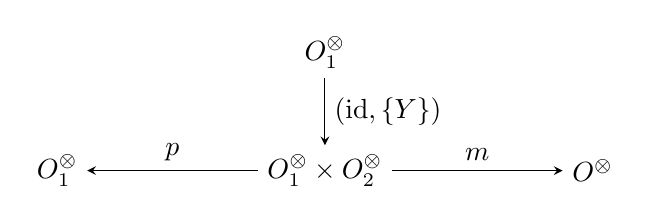
\begin{tikzpicture}[>=stealth,scale=1]
\node (O1) at (0,0) {$O_{1}^{\otimes}$};
\node (P)  at (3.4,0) {$O_{1}^{\otimes}\times O_{2}^{\otimes}$};
\node (O)  at (6.8,0) {$O^{\otimes}$};
\node (T)  at (3.4,1.5) {$O_{1}^{\otimes}$};
\draw[->] (P) -- (O1) node[midway,above] {$p$};
\draw[->] (P) -- (O)  node[midway,above] {$m$};
\draw[->] (T) -- (P)  node[midway,right] {$(\mathrm{id},\{Y\})$};
\end{tikzpicture}
\end{center}
诱导自然函子
\[
\Alg_{O_{2}/O}(\cC)^{\otimes}\to O_{1}^{\otimes}\times_{O^{\otimes}}\cC^{\otimes}.
\]
特别地，我们得到函子
\[
\mathrm{ev}_{Y}\colon\Alg_{O_{2}/O}(\cC)^{\otimes}\to\cC^{\otimes}.
\]
\end{exercise}

\begin{proposition}\label{L26-3.5}（HA.3.2.4.3）
在上述设定下：
\begin{enumerate}[label=(\arabic*),leftmargin=2.4em,itemsep=0.1em]
\item 函子 $\Alg_{O_{2}/O}(\cC)^{\otimes}\to O_{1}^{\otimes}$ 把 $\Alg_{O_{2}/O}(\cC)^{\otimes}$ 展示为 $O_{1}^{\otimes}$ 上的 $\infty$-操作子。此外，$\Alg_{O_{2}/O}(\cC)^{\otimes}$ 中的态射是惰性的，当且仅当
\begin{itemize}[leftmargin=2.2em,itemsep=0.1em]
\item 它在 $O_{1}^{\otimes}$ 中的像是惰性的；
\item 对任意 $Y\in O_{2}$，它在 $\mathrm{ev}_{Y}$ 下的像是惰性的。
\end{itemize}
\item 若 $\cC^{\otimes}\to O^{\otimes}$ 是 $O$-幺半 $\infty$-范畴，则 $\Alg_{O_{2}/O}(\cC)^{\otimes}\to O_{1}^{\otimes}$ 是 $O_{1}$-幺半 $\infty$-范畴。此外，$\Alg_{O_{2}/O}(\cC)^{\otimes}$ 中的态射在 $O_{1}^{\otimes}$ 上是余笛卡尔的，当且仅当对任意 $Y\in O_{2}$，它在 $\mathrm{ev}_{Y}$ 下的像在 $O^{\otimes}$ 上是余笛卡尔的。
\end{enumerate}
\end{proposition}

\begin{example}\label{L26-3.6}
对任意 $\infty$-操作子 $O^{\otimes}$，我们有 $\infty$-操作子映射 $(\mathrm{Comm}\odot O)^{\otimes}\to\mathrm{Comm}^{\otimes}$。由此，对任意 $\infty$-操作子 $\cC^{\otimes}$，存在典范的 $\infty$-操作子 $\Alg_{O}(\cC)^{\otimes}$，它配备到 $\cC^{\otimes}$ 的 $\infty$-操作子映射，且其底层的颜色 $\infty$-范畴是 $\Alg_{O}(\cC)$。此外，若 $\cC$ 是对称幺半的，则 $\Alg_{O}(\cC)$ 也是，且遗忘函子 $\Alg_{O}(\cC)^{\otimes}\to\cC^{\otimes}$ 是对称幺半的。
\end{example}

\begin{exercise}\label{L26-3.7}
在构造~\ref{L26-3.2} 的设定下，当 $O^{\otimes}\coloneqq(O_{1}\odot O_{2})^{\otimes}$ 时，我们有典范等价
\[
\Alg_{O_{1}}(\Alg_{O_{2}}(\cC))\simeq\Alg_{O_{1}\odot O_{2}}(\cC).
\]
\end{exercise}

\begin{proposition}\label{L26-3.8}（HA.3.2.4.7）
设 $\cC^{\otimes}$ 是对称幺半 $\infty$-范畴。则 $\Alg_{\mathrm{Comm}}(\cC)^{\otimes}$ 上的对称幺半结构是余笛卡尔的。特别地，$\Alg_{\mathrm{Comm}}(\cC)$ 承认余积。
\end{proposition}

\begin{remark}\label{L26-3.9}
非形式地说，上述命题说明交换代数的余积由张量积给出。
\end{remark}

\section{$E_{k}$-代数}

\begin{definition}\label{L26-4.1}
设 $k\ge0$ 是非负整数。定义拓扑操作子 ${}^{t}E_{k}^{\otimes}\to\mathrm{Fin}_{*}$，使得：
\begin{itemize}[leftmargin=2.2em,itemsep=0.1em]
\item ${}^{t}E_{k}^{\otimes}$ 中的对象是带标记有限集 $\langle n\rangle$；
\item 从 $\langle m\rangle$ 到 $\langle n\rangle$ 的态射构成的拓扑空间是
\[
\bigsqcup_{\langle m\rangle\xrightarrow{\alpha}\langle n\rangle}\ \prod_{j\in\langle n\rangle^{\circ}}\operatorname{Rect}\bigl(\square^{k}\times\alpha^{-1}(j),\square^{k}\bigr),
\]
其中 $\square\defeq(-1,1)$，而 $\operatorname{Rect}(-,-)$ 是满足下述条件的开嵌入 $\square^{k}\times\alpha^{-1}(j)\to\square^{k}$ 构成的空间：对每个 $i\in\alpha^{-1}(j)$，映射 $f_{i}\colon\square^{k}\to\square^{k}$ 是\textbf{直线嵌入}（rectilinear embedding），即形如
\[
f_{i}(x_{1},\cdots,x_{k})=(a_{1}x_{1}+b_{1},\cdots,a_{k}x_{k}+b_{k})
\]
的映射。
\end{itemize}
令 $E_{k}^{\otimes}$ 为通过函子 $\Cat_{\mathrm{Top}}\to\Cat_{\infty}$ 对应于 ${}^{t}E_{k}^{\otimes}$ 的 $\infty$-操作子。我们称它为 $k$ 维\textbf{小方体 $\infty$-操作子}。
\end{definition}

\begin{exercise}\label{L26-4.2}
$E_{k}^{\otimes}$ 中（活动）$m$ 元运算构成的空间，可以实现为 $\square^{k}$ 中 $m$ 个互异点构成的同伦型。特别地：
\begin{enumerate}[label=(\arabic*),start=0,leftmargin=2.4em,itemsep=0.1em]
\item $E_{k}^{\otimes}$ 是\textbf{带单位的}，即零元运算构成的空间可缩；
\item $E_{k}^{\otimes}$ 是\textbf{约化的}，即一元运算构成的空间可缩；
\item $E_{k}^{\otimes}$ 中二元运算构成的空间同伦于 $S^{k-1}$。
\end{enumerate}
\end{exercise}

\begin{exercise}\label{L26-4.3}
$E_{k}^{\otimes}$ 中（活动）$m$ 元运算构成的空间是 $(k-1)$-连通的，即对 $i<k-1$ 有 $\pi_{i}\simeq0$。
\end{exercise}

\begin{exercise}\label{L26-4.4}
证明上面定义的 $E_{0}^{\otimes}$ 与先前的定义一致：它就是 $\mathrm{Fin}_{*}$ 的由单射态射构成的子范畴。
\end{exercise}

\begin{exercise}\label{L26-4.5}
证明 $E_{1}^{\otimes}\simeq\mathrm{Assoc}^{\otimes}$。
\end{exercise}

\nitem\label{L26-4.6} 对 $0\le k\le k^{\prime}$，我们有 $\infty$-操作子映射 $E_{k}^{\otimes}\to E_{k^{\prime}}^{\otimes}$，它把直线嵌入 $f\colon\square^{k}\to\square^{k}$ 送到 $(f,\id)\colon\square^{k}\times\square^{k^{\prime}-k}\to\square^{k}\times\square^{k^{\prime}-k}$。

\begin{proposition}\label{L26-4.7}（HA.5.1.1.5）
我们有
\[
\colim_{k}E_{k}^{\otimes}\simeq\mathrm{Comm}^{\otimes},
\]
其中余极限在 $\mathrm{Op}_{\infty}$ 中取。特别地，对任意 $\infty$-操作子 $C$，有
\[
\Alg_{\mathrm{Comm}}(C)\simeq\lim_{k}\Alg_{E_{k}}(C).
\]
\end{proposition}

\nitem\label{L26-4.8} 受上述结果启发，我们也记
\[
E_{\infty}^{\otimes}\coloneqq\mathrm{Comm}^{\otimes}.
\]

\begin{construction}\label{L26-4.9}
设 $k,k^{\prime}\ge0$ 是非负整数。我们有函子
\[
{}^{t}E_{k}^{\otimes}\times{}^{t}E_{k^{\prime}}^{\otimes}\to{}^{t}E_{k+k^{\prime}}^{\otimes},
\]
它定义在 $\mathrm{Fin}_{*}\times\mathrm{Fin}_{*}\xrightarrow{\wedge}\mathrm{Fin}_{*}$ 之上，并由 $\square^{k}\times\square^{k^{\prime}}\simeq\square^{k+k^{\prime}}$ 诱导。过渡到 $\infty$-范畴，我们得到函子
\[
E_{k}^{\otimes}\times E_{k^{\prime}}^{\otimes}\to E_{k+k^{\prime}}^{\otimes}.
\]
\end{construction}

\begin{exercise}\label{L26-4.10}
写出上述函子的显式公式，并验证它在每个因子上保持惰性态射。
\end{exercise}

\nitem\label{L26-4.11} 下述结果称为 \textbf{Dunn 加性定理}。

\begin{theorem}\label{L26-4.12}（HA.5.1.2.2）
设 $k,k^{\prime}\ge0$ 是非负整数。函子 $E_{k}^{\otimes}\times E_{k^{\prime}}^{\otimes}\to E_{k+k^{\prime}}^{\otimes}$ 诱导一个等价
\[
(E_{k}\odot E_{k^{\prime}})^{\otimes}\simeq E_{k+k^{\prime}}^{\otimes}.
\]
\end{theorem}

\begin{remark}\label{L26-4.13}
非形式地说，上述定理说明 $E_{k+k^{\prime}}$-代数与「$E_{k^{\prime}}$-代数中的 $E_{k}$-代数」是一样的。
\end{remark}

\begin{corollary}\label{L26-4.14}
设 $k\ge0$ 是非负整数。则 $(E_{k}\odot\mathrm{Comm})^{\otimes}\simeq\mathrm{Comm}^{\otimes}$。
\end{corollary}

\nitem\label{L26-4.15} 下述结果称为 \textbf{Baez--Dolan 稳定化假设}，它由练习~\ref{L26-4.3} 推出。

\begin{proposition}\label{L26-4.16}
设 $\cC$ 是对称幺半 $(n,1)$-范畴。则映射 $E_{k}^{\otimes}\to E_{\infty}^{\otimes}$ 诱导一个等价
\[
\Alg_{E_{\infty}}(\cC)\simeq\Alg_{E_{k}}(\cC),
\]
对任意 $k>n$ 成立。
\end{proposition}

\begin{remark}\label{L26-4.17}
特别地，在普通范畴中，任何超出 $E_{2}$ 的结构都是交换的。
\end{remark}

\nitem\label{L26-4.18} 注意普通范畴自身构成一个 $(2,1)$-范畴。因此，可以存在有趣的、并非对称幺半的 $E_{2}$-幺半普通范畴。

\begin{proposition}\label{L26-4.19}（HA.5.1.2.4）
$E_{2}$-幺半普通范畴恰好就是辫幺半范畴。
\end{proposition}

\begin{remark}\label{L26-4.20}
非形式地说，$E_{2}$ 中二元运算构成的空间同伦于 $S^{1}$，这意味着 $E_{2}$-幺半普通范畴 $\cC$ 给出一个 $\Sigma_{2}$-等变函子 $S^{1}\times\cC\times\cC\to\cC$。对任意点 $s\in S^{1}$，我们得到函子 $\mult_{s}\colon\cC\times\cC\to\cC$ 以及一个等价
\[
\mult_{s}\xrightarrow{\ \simeq\ }\mult_{-s}\circ\sigma,
\]
其中 $\sigma(x,y)\coloneqq(y,x)$。选取从 $1\in S^{1}$ 到 $-1\in S^{1}$ 的一条道路，我们得到等价 $\mult_{1}\xrightarrow{\ \simeq\ }\mult_{-1}$，从而得到等价
\[
\mult_{1}\xrightarrow{\ \simeq\ }\mult_{1}\circ\sigma.
\]
换言之，我们得到函子性同构 $\mult_{1}(x,y)\xrightarrow{\ \simeq\ }\mult_{1}(y,x)$，它们就是相应辫幺半范畴的\textbf{辫态射}。
\end{remark}

\begin{exercise}\label{L26-4.21}
用函子 $S^{1}\times\cC\times\cC\to\cC$ 描述辫的平方。
\end{exercise}

\begin{theorem}\label{L26-4.22}（HA.5.1.1.1）
对 $k\ge1$ 或 $k=\infty$，$\infty$-操作子 $E_{k}^{\otimes}$ 是\textbf{连贯的}。
\end{theorem}

\yizhu{这里的“连贯”是 Lurie 赋予 $\infty$-操作子的一个技术性条件（见 HA.5.1.1.1），与通常所说的“同伦连贯”不是同一概念；译文按 glossary 统一作“连贯”。\textbf{[来源：B]}}

\begin{theorem}\label{L26-4.23}（HA.5.1.3.2）
对 $k\ge1$ 或 $k=\infty$，设 $\cC^{\otimes}\to E_{k}^{\otimes}$ 是与几何实现相容的 $E_{k}$-幺半 $\infty$-范畴。则：
\begin{enumerate}[label=(\arabic*),leftmargin=2.4em,itemsep=0.1em]
\item 对 $A\in\Alg_{/E_{k}}(\cC)$，函子
\[
\Mod^{E_{k}}_{A}(\cC)^{\otimes}\to E_{k}^{\otimes}
\]
是 $E_{k}$-幺半 $\infty$-范畴。
\item 存在典范幺半函子
\[
\Mod^{E_{k}}_{A}(\cC)^{\otimes}\times_{E_{k}^{\otimes}}E_{1}^{\otimes}\to\Mod^{E_{1}}_{A^{\prime}}(\cC\times_{E_{k}}E_{1})^{\otimes},
\]
其中
\[
A^{\prime}\in\Alg_{/E_{1}}(\cC\times_{E_{k}}E_{1})\simeq\Alg^{E_{1}/E_{k}}(\cC)
\]
是复合 $E_{1}^{\otimes}\to E_{k}^{\otimes}\xrightarrow{A}\cC^{\otimes}$。
\end{enumerate}
\end{theorem}

\begin{remark}\label{L26-4.24}
非形式地说，上述定理说明 $E_{k}$-模的相对张量积由底层 $E_{1}$-模的相对张量积给出。
\end{remark}

\appendixsection{因子同调}

\nitem\label{L26-A.1} 给定任意 $E_{k}$-代数 $A$，对任意 $k$-流形 $M$，可以得到一个不变量 $\int_{M}A$，称为 $A$ 在 $M$ 上的\textbf{因子同调}。

\yizhu{“因子同调”（factorization homology）是 Ayala 与 Francis 发展的一种不变量，见本讲参考文献 [AF20]；此处沿用该领域中文文献的译法。\textbf{[来源：A]}}

\nitem\label{L26-A.2} \textbf{建议阅读}\quad HA.5.5.、[AF20]（及其所列参考文献）。

\subsection*{参考文献}
\par\noindent\hangindent=5.2em\hangafter=1 [AF20]\hspace{0.6em}David Ayala and John Francis. A factorization homology primer. In \emph{Handbook of homotopy theory}, pages 39--101. Chapman and Hall/CRC, 2020.
